\ifthenelse{\boolean{papier}}{\clearemptydoublepage}{}
\chapter{Cadre de l’étude}\label{cadre}
\ifthenelse{\boolean{caco}}{}{\pagenumbering{arabic}}
\section{Contexte théorique}
% Introduction à la culture scientifique
Nous évoluons dans une société où la culture scientifique, technique et industrielle (CSTI) occupe une place importante, que cela soit par sa présence quotidienne ou à travers les budgets en recherche et développement (R\&D) qui sont investis chaque année par les entreprises et les gouvernements. Selon un rapport de l’Office parlementaire d’évaluation des choix scientifiques et technologiques \cite{Olivier2014}, bien que la diffusion de la CSTI soit considérée comme un enjeu de politique publique, elle ne semble pas l’être comme une priorité nationale. Afin de maintenir une certaine dynamique en R\&D, l’éducation scientifique a toute son importance. Pour cela, il serait intéressant de savoir quelle est la place que la société accorde à l’éducation et plus particulièrement à l’éducation scientifique.

% Mise en place du socle
Depuis la \citeA{loi2005} la scolarité obligatoire doit garantir à chaque élève les moyens nécessaires à l’acquisition d’un socle commun qui doit permettre la poursuite d’études, la construction d’un avenir personnel et professionnel et préparer à l’exercice de la citoyenneté. La version en vigueur de 2005 à 2013\footnote{À partir du 10~juillet 2013, les grandes compétences du socle ne sont plus énumérées dans cet article de loi : \url{http://www.legifrance.gouv.fr/affichCodeArticle.do?idArticle=LEGIARTI000027682636&cidTexte=LEGITEXT000006071191}} de l’article~\mbox{L122-1-1} du \textit{Code de l’éducation} %\citeA{CodeEdu} 
précise qu’une des grandes compétences du socle est la culture humaniste et scientifique et qu’elle permet le libre exercice de la citoyenneté. Avec le \citeA{DecretSocle} le socle est mis en place et il est inséré au code de l’éducation. Il s’agit d’un contrat social entre l’État et la société. La culture scientifique et technologique devient à elle seule une des grandes compétences du socle. L’élève doit être capable de pratiquer une démarche scientifique, c’est-à-dire qu’il doit être capable d’observer, de se questionner, de formuler une hypothèse et de la valider, d’argumenter et de modéliser de façon élémentaire. Il doit également être capable de manipuler et d’expérimenter en éprouvant la résistance du réel, ce qui se fait entre autres en participant à la conception et à la mise en œuvre de protocoles.

% Introduction de La main à la pâte
Dans \textit{Le socle commun de connaissances et de compétences} \cite[p.~12]{Socle} qui fait partie du code de l’éducation\footnote{Article Annexe suivant l’article D122-3} , il est précisé que: 
\ifthenelse{\boolean{caco}}{\begin{caco}}{\begin{quotation}}Les sciences expérimentales et les technologies ont pour objectif de comprendre et de décrire le monde réel, celui de la nature, celui construit par l’Homme ainsi que les changements induits par l’activité humaine.

% Deuxième § de la citation
Leur étude contribue à faire comprendre aux élèves la distinction entre faits et hypothèses vérifiables d’une part, opinions et croyances d’autre part. Pour atteindre ces buts, l’observation, le questionnement, la manipulation et l’expérimentation sont essentiels, et cela dès l’école primaire, dans l’esprit de l’opération \og La main à la pâte \fg{} qui donne le gout des sciences et des techniques dès le plus jeune âge.
\ifthenelse{\boolean{caco}}{\end{caco}}{\end{quotation}}

%La main à la pâte
L’opération \og La main à la pâte \fg{} a été lancé en 1995 par le physicien Georges Charpak avec la collaboration du ministère de l’Éducation nationale et s’est inspiré de l’opération \og hands on \fg{} (travail de terrain) mise en pratique dans les écoles défavorisées de Chicago par le physicien Leon Lederman. Le rapport de l’Office parlementaire d’évaluation des choix scientifiques et technologiques sur \emph{Faire connaitre et partager les cultures scientifiques, techniques et industrielles : un impératif}, considère \og La main à la pâte \fg{} comme le plus célèbre des programmes de rénovation de l’enseignement des sciences au primaire \cite{Olivier2014}.

% La démarche d’investigation
La démarche préconisée par \og La main à la pâte \fg{} s’intitule la démarche d’investigation. Son but est de \og permettre aux enfants de construire les connaissances souhaitées en leur permettant d’exprimer leurs idées, d’expliciter leur raisonnement, de tester leurs hypothèses et de chercher à être rigoureux \fg{} \cite[p.~9]{Saltiel2005}. Pour cela, il est important que les élèves s’approprient la question initiale, expérimentent par eux-mêmes, savent ce qu’il faut observer ou à chercher et que les élèves interagissent entre eux aussi bien à l’oral qu’à l’écrit (écrire pour les autres). L’investigation réalisée par les élèves peut s’appuyer sur diverses méthodes : l’expérimentation, la recherche documentaire, l’observation et la modélisation.

%Schéma
La démarche d’investigation pourrait être résumé en un schéma (%Dominique Rojat, IGEN SVT, 
cf. fig.~\ref{demarcheInvestigation}% p.~\pageref{demarcheInvestigation}
) que l’on trouve dans le \textit{Guide de Découverte : Un enseignement intégré de science et technologie au collège (6\ieme{} et 5\ieme)} \cite[p.~65]{Lena2011} et sur le site\footnote{\url{http://www.fondation-lamap.org/fr/page/17793/la-demarche-dinvestigation}} de la Fondation \textit{La main à la pâte}.
\begin{figure}[h!tbp]
%\begin{figure}[htbp]
  \centering
  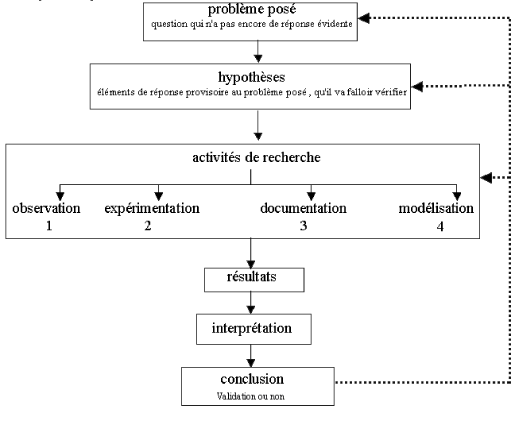
\includegraphics[width=\textwidth]{demarcheInvestigation.png}
  \caption{La démarche d’investigation (d’après Dominique Rojat, IGEN SVT)}
  \label{demarcheInvestigation}
\end{figure}
%Démarche dès la maternelle
Cette démarche serait réalisable dès la maternelle. Pour preuve, voici un extrait de l’audition de M. Georges Charpak devant la commission des affaires culturelles, familiales et sociales sur l’enseignement des disciplines scientifiques dans le primaire et le secondaire qui a eu lieu le 20~décembre 2005:
\ifthenelse{\boolean{caco}}{\begin{caco}}{\begin{quotation}}J’ai fait l’expérience d’emmener un chef d’État d’Amérique latine, en compagnie de l’ambassadeur de France, dans une classe de dernière année d’école maternelle où il a constaté qu’après trois leçons sur la densité, les élèves de cinq et six ans savaient mieux que lui, que tous les membres de son cabinet et que l’ambassadeur ce qui, d’un pamplemousse ou d’un haricot, flottait ou coulait une fois dans l’eau\dots{} Il a vu qu’ils avaient aussi appris à s’exprimer, qu’ils tenaient un cahier d’expériences. \cite[p.~157]{Rolland2006}
\ifthenelse{\boolean{caco}}{\end{caco}}{\end{quotation}}

% Littérature
Bien que cette démarche pourrait sembler plus délicate à mettre en œuvre à l’école maternelle qu’au primaire, il est possible de trouver une certaine littérature avec des projets de séquences d’enseignement. \citeA{Sacy2000} dans son livret destiné à des expériences sur l’eau et l’air en petite section précise à la page~4 qu’\og avec les connaissances de base de chacun et avec le vocabulaire des enfants, la technologie permet d’amener l’enfant à regarder autrement les objets et les éléments de sa vie quotidienne \fg{} ce qui est en accord avec la philosophie des \emph{Programmes de l’école primaire} de 1995 : \og l’enseignant-e d’école maternelle doit susciter toutes les occasions d’une découverte active du monde et de ses représentations. \fg{} \cite[p.~3]{Sacy2000}. De même, \citeA{Sanchez2012} qui ont construit 23~séquences pour des enfants du cycle~1, sont convaincus que \og à de rares exceptions près n’importe quel concept scientifique peut être abordé avec chaque enfant, à n’importe quel âge, à partir de situations adaptées \fg{} (p.~4). C’est en accord avec ce que dit \citeA[p.~8]{Coquide2002} :
\ifthenelse{\boolean{caco}}{\og}{\begin{quotation}}Si les petits ne possèdent pas encore certains types d’organisation propre à la pensée scientifique ou aux démarches technologiques, ils n’en développent pas moins une intense activité intellectuelle, nourrie par un besoin d’agir, de connaitre, de se questionner sur l’environnement qui les entoure\dots{}
\ifthenelse{\boolean{caco}}{\fg{}}{\end{quotation}}
Et en parlant de ce livre, \citeA[p.~47]{Drouard2008} précise:
\ifthenelse{\boolean{caco}}{\begin{caco}}{\begin{quotation}}Les auteurs rappellent que de vraies hypothèses propres à la méthode hypothético-déductive ne sont à envisager qu’au cycle~3 et que les \og hypothèses\fg{} ne sont pas vraiment de même nature au cycle~2. C’est pourquoi on parle dans cet ouvrage, pour la maternelle (et aussi pour le cycle~2), de situations déclenchantes et de questions inductrices, et non de situations de départ et de problèmes.
\ifthenelse{\boolean{caco}}{\end{caco}}{\end{quotation}}

% Développement du langage
Dans les \textit{Horaires et programmes d’enseignement de l’école primaire} \cite{BO2008} il est dit que l’objectif essentiel de l’école maternelle est l’acquisition d’un
langage oral riche, organisé et compréhensible par l’autre. Il existe une relation entre l’exploration du monde et le développement du langage. Selon les documents d’accompagnement des anciens programmes de 2002 \cite{Adam2005} l’exploration du monde est fondamentale et préalable à la naissance du langage. C’est une des raisons pour laquelle l’enfant doit découvrir le monde de façon active tel qu’il peut être perçu. À la fin de l’école maternelle, aucun élève ne peut avoir construit de manière stable une logique scientifique, générale et structurée. Cela n’empêche pas d’aboutir à des formulations générales et structurées à l’école maternelle.

% Le langage
En ce qui concerne le langage, \citeA{Bisault2005} a réalisé une étude sur l’argumentation dans l’enseignement des sciences en petite et moyenne section de maternelle. Il n’y a pas seulement la communication verbale qui jour un rôle dans les apprentissages, mais également les dessins, les schémas, les gestes et les actions partagées : \og Les actions et observations réalisées par quelques élèves ont été largement intégrées par les autres élèves même si elles n’ont pas toujours été systématiquement verbalisées \fg{} (p.~137).


\section{Contexte professionnel}
Cette étude est faite dans le cadre de la deuxième année du master Métiers de l’enseignement, de l’éducation et de la formation lors d’un stage d’observation et de pratique accompagnée à l’école maternelle Jean-Henri Fabre à Avignon du 7~octobre au 17~décembre~2014 et du 3~février au 20~mai~2015 dans une classe mixte de petite et moyenne section avec respectivement 19 et 7~élèves. Durant la première partie de ce stage, j’ai pu construire, mettre en œuvre et animer une séquence d’enseignement et d’apprentissage sur la germination des graines. %En 2011, l’école faisait partie du programme Écoles, collèges et lycées pour l’ambition, l’innovation et la réussite\footnote{\url{http://cache.media.education.gouv.fr/file/27/68/6/eclair_liste_etablissement_184686.pdf}}.


\section{État des lieux de la question}
% Rapport Sarmant
Selon le \emph{Rapport sur l’opération \og La main à la pâte \fg{} et l’enseignement des sciences à l’école primaire} de l’inspection générale de l’Éducation nationale \cite{Sarmant1999}, 27 classes ont été visitées du 19~mars au 4~juin 1999, réparties dans des départements fortement ou peu impliqués dans l’opération. Une différence pédagogique a été observée entre les deux types de départements : \og Les démarches pratiquées dans les classes sont nettement différentes: descriptive et affirmative dans les départements non engagés, impliquant l’activité de l’élève et sa réflexion dans les autres \fg{} (p.~5). Néanmoins, deux types de dérives ont pu être observées, la dérive du \og tout méthodologique \fg{} où l’acquisition de connaissances est un objectif mineur et la dérive du \og tout technologique \fg{} où l’activité consiste à réaliser un objet, sans autre problématique.

% Rapport IGEN
Il ne faut pas oublier, comme nous le rappelle un rapport de l’\citeA{IGEN2001} sur \textit{L’enseignement des sciences et de la technologie à l’école primaire}, que l’enseignement des sciences et de la technologie est peu pratiqué à l’école et qu’il y a très peu de classes élémentaires où cet enseignement s’appuie sur des expériences réalisées par les élèves. De plus, comme le nous remémore clairement les anciens \textit{Horaires et programmes d’enseignement de l’école primaire} \cite[p.~31]{BO2002}, il ne faut pas faire des expériences juste pour faire des expériences : 
\ifthenelse{\boolean{caco}}{\og}{\begin{quotation}}
Issue d’un questionnement provenant le plus souvent de l’activité des enfants, l’investigation menée en maternelle n’est pas conduite uniquement pour elle-même : elle débouche sur des savoir-faire et des connaissances. Même très élémentaires, ces derniers constituent un progrès important pour l’élève.
\ifthenelse{\boolean{caco}}{\fg{}}{\end{quotation}}
C’est ainsi que le document d’accompagnement \textit{Enseigner les sciences à l’école : outil pour la mise en œuvre des programmes 2002 : cycles~1 et 2} \cite{CNDP2002} a été écrit avec l’ambition d’accompagner les enseignants dans le développement d’un enseignement basé sur le questionnement et sur l’expérimentation par les élèves eux-mêmes.

% BO2008
Le 9~juin 2008, les horaires d’enseignement à l’école élémentaire par domaine disciplinaire et les programmes d’enseignement de l’école sont fixés par arrêté ministériel et sont publiés au journal officiel le 17~juin ; ce sont les \textit{Horaires et programmes d’enseignement de l’école primaire} \cite{BO2008}. À l’école maternelle, cycle des apprentissages premiers, il y a un domaine intitulé \emph{Découvrir le Monde} qui devient \emph{Découverte du monde} au cycle des apprentissages fondamentaux et \emph{Sciences expérimentales et technologie} au cycle des approfondissements. En ce qui concerne les horaires, il n’y a pas un horaire spécifique à \emph{Découvrir le Monde} en maternelle, alors qu’à l’école élémentaire la \og découverte du monde \fg{} au cycle~2 et les \og sciences expérimentales et technologie \fg{} représentent 9~\% de la durée annuelle des enseignements. %Maintenant que nous avons la place que représentent les sciences dans les sciences, on peut se demander quelle démarche est préconisée pour l’enseigner.

% Nouveaux programmes
Dans les \emph{Recommandations pour la mise en œuvre des programmes de l’école élémentaire} du \citeA{CSP2014} du 15~mai 2014, il est précisé qu’en sciences expérimentales et technologie (cycle des approfondissements), les connaissances et les compétences doivent être acquises dans le cadre d’une démarche d’investigation qui développe la curiosité, la créativité, l’esprit critique et l’intérêt pour le progrès scientifique et technique. Cependant, il n’est pas exigé que chacune des étapes de la démarche d’investigation soit systématiquement abordée lors de l’étude de chaque thème du programme. Le terme \og démarche d’investigation \fg{} n’est utilisé par le Conseil supérieur des programmes (CSP) que pour le cycle des approfondissements. Pour le cycle des apprentissages fondamentaux, le CSP ne donne aucune recommandation. Dans le \emph{Projet de programme et recommandations pour l’école maternelle} \cite{CSP2014b} du 3~juillet 2014, il est mentionné que les enfants sont conduits vers un questionnement qui s’ouvre et s’affine au fur et à mesure qu’ils agissent, essaient, constatent, formulent, représentent et réessaient. L’enseignant les aide à construire, trouver, comprendre des principes ou des généralités à travers des manipulations et des expériences. Un des objectifs est de leur donner l’habitude de regarder différemment ce qui leur paraissait auparavant familier, en devenant curieux, en s’interrogeant, en faisant des hypothèses, en comparant et contrastant. Pour la maternelle, le CSP parle d’expériences, mais pas de démarche d’investigation, ce qui n’est pas le cas du ministère de l’Éducation nationale de l’Enseignement supérieur et de la Recherche qui précise sur son site internet\footnote{\url{http://www.education.gouv.fr/cid54197/l-enseignement-des-sciences.html}} que \og dès l’école maternelle, les enfants sont initiés à la démarche d’investigation qui développe la curiosité, la créativité, l’esprit critique et l’intérêt pour le progrès scientifique et technique.\fg{} Par conséquent, on peut se demander quelle est la place de la démarche d’investigation en maternelle.

Le 26~mars 2015 est publié au Bulletin officiel de l’Éducation nationale le \textit{Programme d’enseignement de l’école maternelle} \cite{BO2015}. Selon ce programme, les enseignements sont organisés en cinq domaines d’apprentissage. Un de ses cinq domaines s’intitule \og Explorer le monde \fg{}, et il est stipulé que chaque domaine \og doit trouver sa place dans l’organisation du temps quotidien \fg{}. Le domaine \og Explorer le monde \fg{} se définit en deux sous-domaines : \og Se repérer dans le temps et l’espace \fg{} et \og Explorer le monde du vivant, des objets et de la matière \fg{} où il est précisé que \og l’enseignant propose des activités qui amènent les enfants à observer, formuler des interrogations plus rationnelles, construire des relations entre les phénomènes observés, prévoir des conséquences, identifier des caractéristiques susceptibles d’être catégorisées \fg{} afin de \og les aider à découvrir, organiser et comprendre le monde qui les entoure \fg{}. Bien que la démarche d’investigation ne soit pas spécifiée, elle répond aux exigences du programme.

Pour finir, bien qu’il ne s’agisse pas d’un document spécifique à la maternelle, on remarque que la démarche d’investigation fait partie du tout nouveau \emph{Socle commun de connaissances, de compétences et de culture} \cite{Socle2015} où l’élève doit découvrir la nature environnante par une approche scientifique qui est fondée sur l’observation, la manipulation et l’expérimentation.

\section{Intérêt de la question}
Les \textit{Horaires et programmes d’enseignement de l’école primaire} \cite{BO2008} parlent de démarche d’investigation, en générale et plus précisément pour le cycle~3. La recommandation du ministère de l’Éducation nationale, de l’Enseignement supérieur et de la Recherche est que les enfants soient initiés à cette démarche dès la maternelle. Dans quelle mesure l’enseignement de cette démarche se fait-il en maternelle ? La réponse à cette question pourra permettre un premier état des lieux des pratiques enseignantes, ce qui peut donner des repères aux (jeunes) enseignants de maternelle.